\section{Results}
\label{SECIV}\label{sec:results}

We tested the new detection method with mock Advanced \textsc{ligo} having a power spectrum prescribed by the ``zero detuning, high power'' noise model in \cite{Shoemaker:2009p9770}.  Colored Gaussian noise is generated by passing 5 independent realizations of white Gaussian noise sampled at 16384 Hz through \textsc{iir} filters with coefficients shown in equation~(\ref{eq:iirbank}) below, then summing the filters' outputs.  This carefully designed filter bank reproduces the noise model very faithfully, but since it is composed of \textsc{iir} filters it can produce mock data in realtime very cheaply.

\begin{eqnarray}
\label{eq:iirbank}
x_i &[n] \sim& \mathcal{N}[0, 1] \quad \forall \, i, n \nonumber\\\noalign{\vskip 2mm}
y_1 &[n] =& \left(4 \times 10^{-28}\right) x_1[n] - y_1[n-1] + 2 \cdot .99995 \cos \left(\frac{2\pi \cdot 9.103}{16384}\right) y_1[n-2] - .99995^2 y_1[n-3] \nonumber\\\noalign{\vskip 2mm}
y_2 &[n] =& \left(1.1 \times 10^{-23}\right) (x_2[n] - x_2[n-1]) \nonumber\\\noalign{\vskip 2mm}
y_3 &[n] =& \left(4 10^{-27}\right) x_3[n] - y_3[n-1] + 2 \cdot .999 y_3[n-2] - .999^2 y_3[n-3] \nonumber\\\noalign{\vskip 2mm}
y_4 &[n] =& \left(4 \times 10^{-26}\right) x_4[n] - y_4[n-1] + 2 \cdot .87 \cos \left(\frac{2\pi \cdot 50}{16384}\right) y_4[n-2] - .87 ^ 2 y_4[n-3] \nonumber\\\noalign{\vskip 2mm}
y_5 &[n] =& \left(6.5 \times 10^{-24}\right) x_5[n] - y_5[n-1] - .45 \cdot 2 y_5[n-2] - .45 ^ 2 y_5[n-3] \nonumber\\\noalign{\vskip 2mm}
\; y &[n] =& \frac{3\sqrt{16384}}{4} \left(y_1[n] + y_2[n] + y_3[n] + y_4[n] + y_5[n]\right)
\end{eqnarray}

\begin{itemize}
\item 1 day of simulated $h(t)$.
\item $h(t)$ has power spectrum \sout{prescribed for ``zero detuning, high power'' model in \cite{Shoemaker:2009p9770}} that somewhat resembles initial \textsc{ligo} noise models
\item $h(t)$ generated by passing white, Gaussian noise through a bank of \textsc{iir} filters
\item 1 noninjections run
\item 10 injections runs
\item injections are distributed uniformly in log distance, uniformly in sky location and binary orientation
\item injections are reweighted to be uniformly distributed in volume
\item injections are 80$\pm$20 seconds apart
\item there are $\approx$ 10k injections
\end{itemize}

\begin{figure}[htbp]
\begin{center}
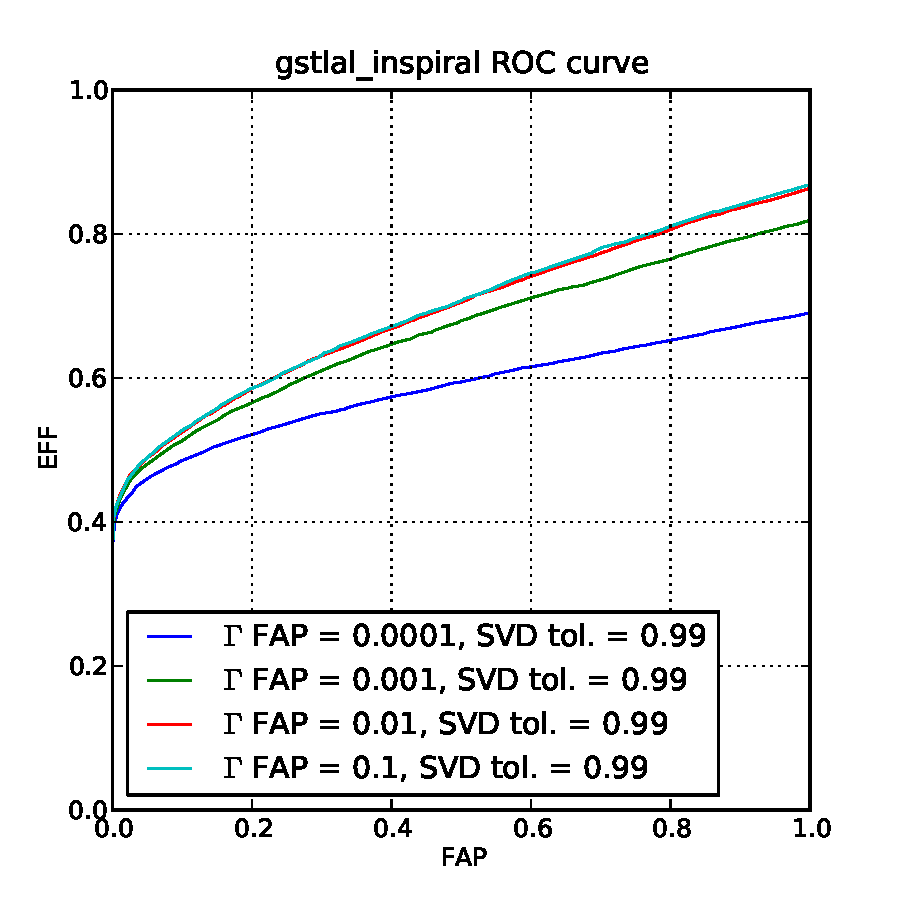
\includegraphics[scale=0.4]{figures/roc_99.pdf}
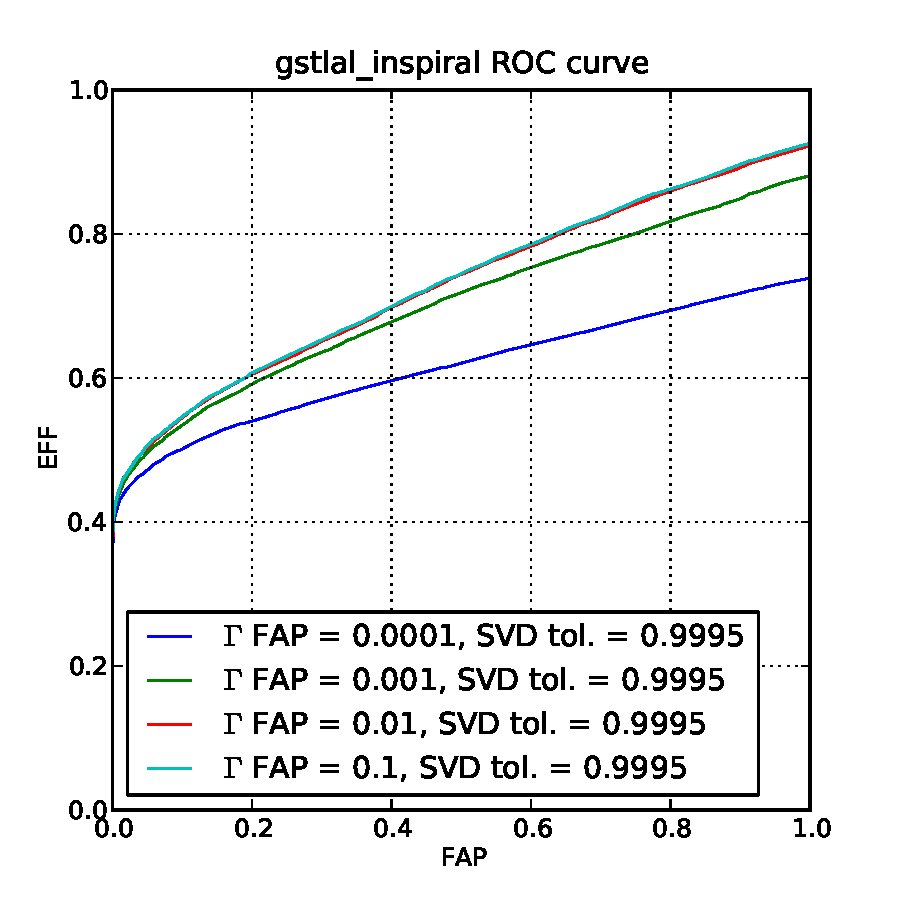
\includegraphics[scale=0.4]{figures/roc_9995.pdf}
\caption{Receiver operating characteristic (\textsc{roc}) curve of detection efficiency (\textsc{eff}) versus false alarm probability (\textsc{fap}).}
\label{fig:roc}
\end{center}
\end{figure}
